% To je predloga za poročila o domačih nalogah pri predmetih, katerih
% nosilec je Blaž Zupan. Seveda lahko tudi dodaš kakšen nov, zanimiv
% in uporaben element, ki ga v tej predlogi (še) ni. Več o LaTeX-u izveš na
% spletu, na primer na http://tobi.oetiker.ch/lshort/lshort.pdf.
%
% To predlogo lahko spremeniš v PDF dokument s pomočjo programa
% pdflatex, ki je del standardne instalacije LaTeX programov.

\documentclass[a4paper,11pt]{article}
\usepackage{a4wide}
\usepackage{fullpage}
\usepackage[utf8x]{inputenc}
\usepackage[slovene]{babel}
\selectlanguage{slovene}
\usepackage[toc,page]{appendix}
\usepackage[pdftex]{graphicx} % za slike
\usepackage{setspace}
\usepackage{color}
\definecolor{light-gray}{gray}{0.95}
\usepackage{listings} % za vključevanje kode
\usepackage{hyperref}
\renewcommand{\baselinestretch}{1.2} % za boljšo berljivost večji razmak
\renewcommand{\appendixpagename}{Priloge}

\lstset{ % nastavitve za izpis kode, sem lahko tudi kaj dodaš/spremeniš
language=Python,
basicstyle=\footnotesize,
basicstyle=\ttfamily\footnotesize\setstretch{1},
backgroundcolor=\color{light-gray},
}

\title{GLASOVANJE ZA PESEM EVROVIZIJE}
\author{Tomaž Tomažič (63100281)}
\date{\today}

\begin{document}

\maketitle

\section{Uvod}

Cilj naloge je bil ugotoviti ali pri glasovanju za pesem evrovizije posamezne države glasujejo pristransko in pri tem favorizirajo nastopajoče iz bljižnjih ali sorodnih držav.

\section{Podatki}

Na voljo so podatki iz preteklih let glasovanj za posamezne države iz polfinala in finala. Iz finala je bilo na voljo 291 primerkov iz polfinala pa 173. Finale imajo 63 atributov, polfinale pa 61. Dejasnko uporabnih podatkov za to nalogo je bilo 13 manj, torej 50 na primerek.
Sam sem programsko analiziral le podatke finalov, ker je več primerkov in je v nih več držav. Torej nekatere države avtomatsko pridejo v finale in preskočijo polfinale.

\section{Metode}

Nalogo sem rešil tako da sem podatke uvozil iz .csv datoteke. Glede na posamezno državo sem naredil povprečje iz vseh let skupaj. S tem sem dobil bolj pregledno sliko podatkov. Tega mi načeloma nebi bilo treba delati, vendar statistično gledano odstopanja ne bi smela biti velika.
Zatem sem podatke transponiral, kar mi je omogočilo delo za naprej, računanje razdalje med državami. Definiral sem razred bicluster, v katerem sem lahko v atribut list shranil države pripadajoče skupine. V metodi hcluster je vsa logika za hierarhično združevanje držav v skupine. Na začetku je vsaka država ena skupina. Potem pa se glede na najmanjšo povprečno razdaljo navidezno združita dve skupini v eno. Torej v vsaki iteraciji je ena skupina manj. Za računanje razadalje med skupinami mi omogča metoda distancebetweengroups ki deluje na principu average linkage. To je povprečna razdalja med vsemi pari primerov iz dveh skupin:

\begin{equation} 
d(Cu,Cv)= 
\frac{\sum\limits_{a\in Cu} \sum\limits_{b\in Cv} d(a, b)}
{|Ca||Cb|} 
\end{equation}


Za razdaljo med posameznima državama pa sem uporabil metodo evklidDistance ki vrne evklidsko razdaljo kot mero različnosti. Pomembno je, da sem dele kjer podatka ni bilo izpustil, saj si bi drugače pokvaril pravo razdaljo. Formula za evlkidsko razadljo je:

\begin{equation}
\sqrt{ 
\sum\limits_{i=1}^{m}(a_{i}-b_{i})^{2}
}
\end{equation}


Za izris dendrograma sem potreboval še ostale metode: drawdendrogram, getheight, getdepth in drawnode. Te sem prepisal iz knjige Programming Collective Intelligence in preuredil za moje potrebe. Na koncu program ustvari sliko dendrograma~\ref{slika1}. Za lažjo ugotovitev pravilnih rezultatov sem dodal zraven države v oklepaje v katero regijo država spada.

\begin{figure}[htbp]
\begin{center}
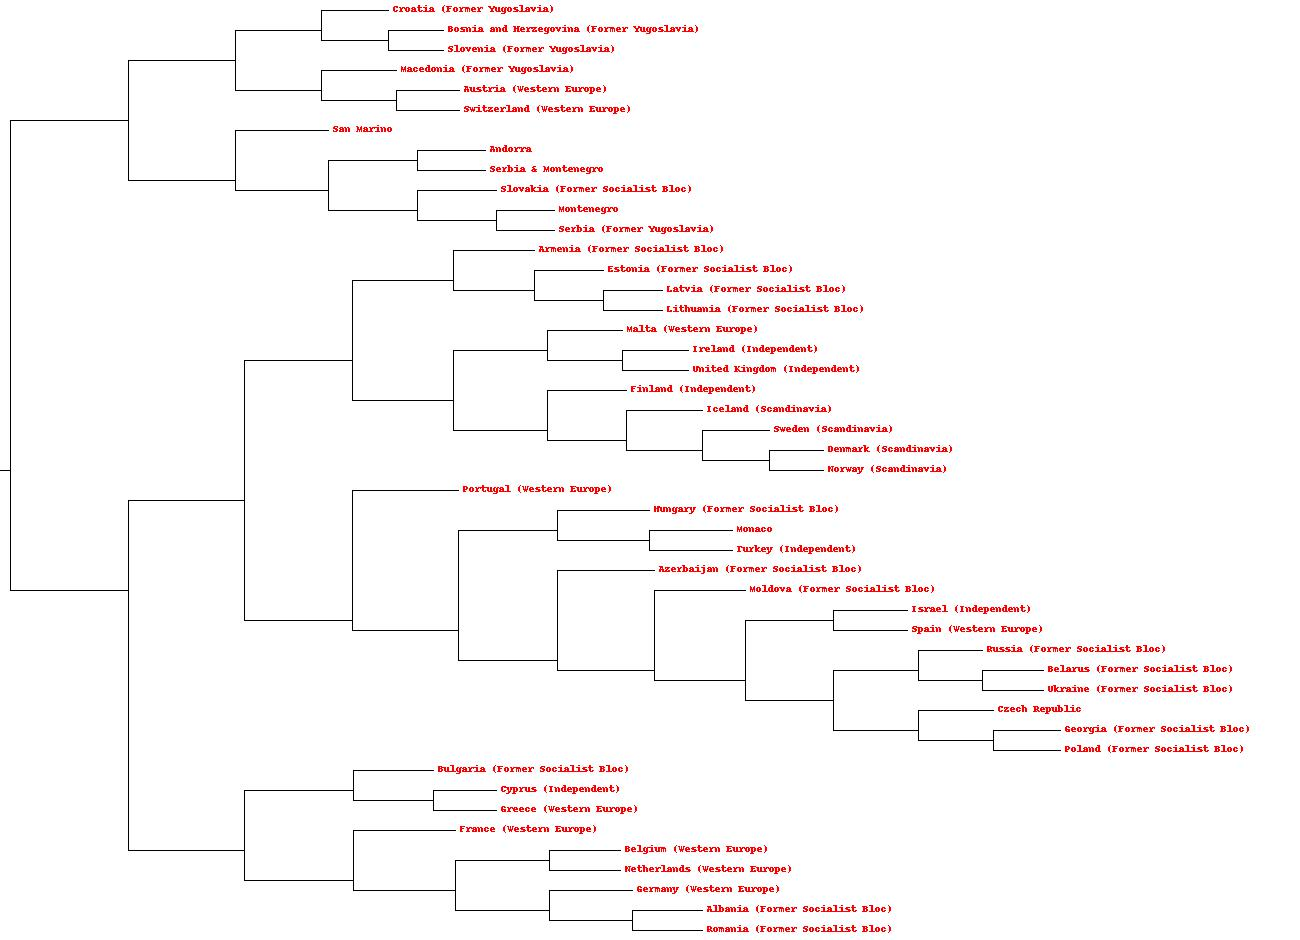
\includegraphics[scale=0.3]{final-dendrogram.jpg}
\caption{Slika je dendrogram ki prikazuje kako je program združil posamezne države v skupine.}
\label{slika1}
\end{center}
\end{figure}

\section{Rezultati}

Rezultati so jasno razvidni iz same slike~\ref{slika1} dendrograma in tako tudi najbolj razumljivi.

Videti je da posamezne države glasujejo pristransko in pri tem favorizirajo nastopajoče iz bljižnjih ali sorodnih držav. Najbolj izrazito je to kjer so skandinavske države skupaj (Finska, Islandija, Švedska, Norveška, Danska). Lepo se vidi tudi v socialističnem bloku (Rusija, Belosrusija, Ukrajina, Poljska) in ostalih skupinah: blok bivše Jugoslavije (Slovenija, Bosna in Hercegovina, Makedonija) in blok zahodne evrope(Nemčija, Nizozemska, Belgija, Francija). Program torej smiselno razvrsti države v skupine

\section{Izjava o izdelavi domače naloge}

Domačo nalogo in pripadajoče programe sem izdelal sam.

\appendix
\appendixpage

\section{\label{app-code}Programska koda}

Celotna koda v Pythonu:

\begin{lstlisting}
from PIL import Image,ImageDraw
import csv
filename="eurovision-final.csv"
indent = 16 \#where interesting data begins
inputfile=csv.reader(open(filename), dialect='excel')
linelist = [line for line in inputfile] \#save in 2D array
firstline=linelist.pop(0) \#first row is not really data
firstline = [f.strip() for f in firstline]
allcountrys=firstline[indent:63] \#first row is saved for later transponation

\# remove unnecessary space
\# map \{name -> region\} to add to final image for easier matching
region=\{\}
for a in range(len(linelist)):
    for b in range(len(linelist[a])):
        linelist[a][b]=linelist[a][b].strip()
    region[linelist[a][1]]=linelist[a][2]


\# merge all rows of same countrys as average to list avgcountrylist
avgcountrylist=[]
set=[] \#create set of
for i in linelist:
    \#one country of all years saved in tmp
    tmp = [j for j in linelist if i[1]==j[1] and i[1] not in set]

    if (tmp):
        tmpvektor=[0]*47
        tmpavgvektor=[0]*47
        for k in tmp:
            for l in range(47):
                if (k[l+indent]):
                    tmpvektor[l]+=int(k[l+indent])
                    tmpavgvektor[l]+=1

        tmpvektor=[(tmpvektor[a]*1.0)/tmpavgvektor[a] if tmpavgvektor[a]>0 else ''  for a in range(len(tmpvektor))]
        set.append(i[1])
        i[indent:63]=tmpvektor
        avgcountrylist.append(i)

\# remove unnecessary data from rows
for i in range(len(avgcountrylist)):
    name = avgcountrylist[i][1]
    for j in range(0,indent):
        avgcountrylist[i].pop(0)
    avgcountrylist[i].insert(0,name)

\# add first meta row
countrys=['']+firstline[indent:63]
avgcountrylist.insert(0,countrys)

\# transpose data in cut
transposed= [list(i) for i in zip(*avgcountrylist)]
cut = transposed[1:]
cut =[a[1:] for a in cut]

\# save new data in countrymap dict to access it when calculating distance between groups
countrymap = \{\}
for a in transposed[1:]:
    countrymap[a[0]]=a[1:]

\# create class which allow us to make groups. In list property are saved all countrys of this group. Also we have left and right to be able to draw dendrogram
class bicluster:
    def \_\_init\_\_(self,left=None,right=None,distance=0.0,id=None,list=[]):
        self.left=left
        self.right=right
        self.id=id
        self.distance=distance
        self.list=list

def evklidDistance(a,b):
    '''
    Calculate distance between two vectors
    '''
    sum=0
    for i,j in zip(a,b):
        if not i and not j:
            sum=sum
        elif not j and i:
            sum+=float(i)
        elif not i and j:
            sum+=float(j)
        else:
            sum+=pow((float(i)-float(j)),2)
    return pow(sum,0.5)

def distancebetweengroups(lista,listb):
    '''
    Calculate distance between two groups
    '''
    avgdist=0
    for a in lista:
        for b in listb:
            avgdist+=evklidDistance(countrymap[a],countrymap[b])
    if lista and listb:
        return (avgdist*1.0)/(len(lista)*len(listb))
    return 0

def hcluster(rows):
    '''
    Adding countrys to groups until one final "unvisible" group. Return final group. From here we can access left and right node.
    '''
    distances=\{\}
    currentclustid=-1
    \# Clusters are initially just the rows
    clust=[bicluster(id=i,list=[allcountrys[i]]) for i in range(len(rows))]
    while len(clust)>1:
        lowestpair=(0,1)
        closest=distancebetweengroups(clust[0].list,clust[1].list)
        \# loop through every pair looking for the smallest distance
        for i in range(len(clust)):
            for j in range(i+1,len(clust)):
                 \# distances is the cache of distance calculations
                if (clust[i].id,clust[j].id) not in distances:
                    distances[(clust[i].id,clust[j].id)]=distancebetweengroups(clust[i].list,clust[j].list)

                d=distances[(clust[i].id,clust[j].id)]

                if d<closest:
                    closest=d
                    lowestpair=(i,j)

        \# create the new cluster
        newcluster=bicluster(
            left=clust[lowestpair[0]],
            right=clust[lowestpair[1]],
            distance=closest,
            id=currentclustid,
            list = clust[lowestpair[0]].list+clust[lowestpair[1]].list
        )
        \# cluster ids that weren't in the original set are negative
        currentclustid-=1
        del clust[lowestpair[1]]
        del clust[lowestpair[0]]
        clust.append(newcluster)
    return clust[0]

def getheight(clust):
    \# Is this an endpoint? Then the height is just 1
    if clust.left==None and clust.right==None: return 1
    \#if clust.left==None and clust.right==None: return 1
    \# Otherwise the height is the same of the heights of
    \# each branch
    return getheight(clust.left)+getheight(clust.right)

def getdepth(clust):
    \# The distance of an endpoint is 0.0
    if clust.left==None and clust.right==None: return 0
    \# The distance of a branch is the greater of its two sides
    \# plus its own distance
    return max(getdepth(clust.left),getdepth(clust.right))+clust.distance

def drawdendrogram(clust,labels,jpeg='clusters.jpg'):
    \# height and width
    h=getheight(clust)*20
    w=1200
    depth=getdepth(clust)
    \# width is fixed, so scale distances accordingly
    scaling=float(w-150)/depth
    \# Create a new image with a white background
    img=Image.new('RGB',(w+100,h),(255,255,255))
    draw=ImageDraw.Draw(img)
    draw.line((0,h/2,10,h/2),fill=(0,0,0))
    \# Draw the first node
    drawnode(draw,clust,10,(h/2),scaling,labels)
    img.save(jpeg,'JPEG')

def drawnode(draw,clust,x,y,scaling,labels):
    if clust.id<0:
        h1=getheight(clust.left)*20
        h2=getheight(clust.right)*20
        top=y-(h1+h2)/2
        bottom=y+(h1+h2)/2
        \# Line length
        ll=clust.distance*scaling
        \# Vertical line from this cluster to children
        draw.line((x,top+h1/2,x,bottom-h2/2),fill=(0,0,0))
        \# Horizontal line to left item
        draw.line((x,top+h1/2,x+ll,top+h1/2),fill=(0,0,0))
        \# Horizontal line to right item
        draw.line((x,bottom-h2/2,x+ll,bottom-h2/2),fill=(0,0,0))
        \# Call the function to draw the left and right nodes
        drawnode(draw,clust.left,x+ll,top+h1/2,scaling,labels)
        drawnode(draw,clust.right,x+ll,bottom-h2/2,scaling,labels)
    else:
        \# If this is an endpoint, draw the item label
        draw.text((x+5,y-7),labels[clust.id],(255,0,0))

\#add to countrys region
for i in range(len(countrys)-1):
    if region.has\_key(countrys[i+1].strip()):
        countrys[i+1]=countrys[i+1]+' ('+region[countrys[i+1].strip()]+ ') '

drawdendrogram(hcluster(cut),countrys[1:],jpeg='final-dendrogram.jpg')
\end{lstlisting}

\end{document}
